\documentclass{hw}
\usepackage{rubylatex}

\begin{document}

In this document, we want to include some cool pictures of cats. But it can be annoying to
continually save pictures, and I like variety, so I'll just pull them from the web.

\begin{rbtex}
require 'open-uri'

links = [
    'http://i.imgur.com/4Nsl5mo.jpg',
    'http://i.imgur.com/xGmX4h3.jpg',
    'http://i.imgur.com/U7vFDsE.jpg',
    'http://i.imgur.com/65TUMwc.jpg',
    'http://i.imgur.com/SpCbHBI.jpg',
    'http://i.imgur.com/4clqUdj.jpg',
    'http://i.imgur.com/YNTFOXs.jpg',
    'http://i.imgur.com/yhbag0Z.jpg',
    'http://i.imgur.com/IUfsijF.jpg',
    'http://i.imgur.com/0FODiod.jpg',
    'http://i.imgur.com/EuAsA4S.jpg'
]

link = links.sample
open(link) {|image|
    File.open('picture.png','w+') do |f|
        f.puts image.read
    end
}

\end{rbtex}
\begin{center}
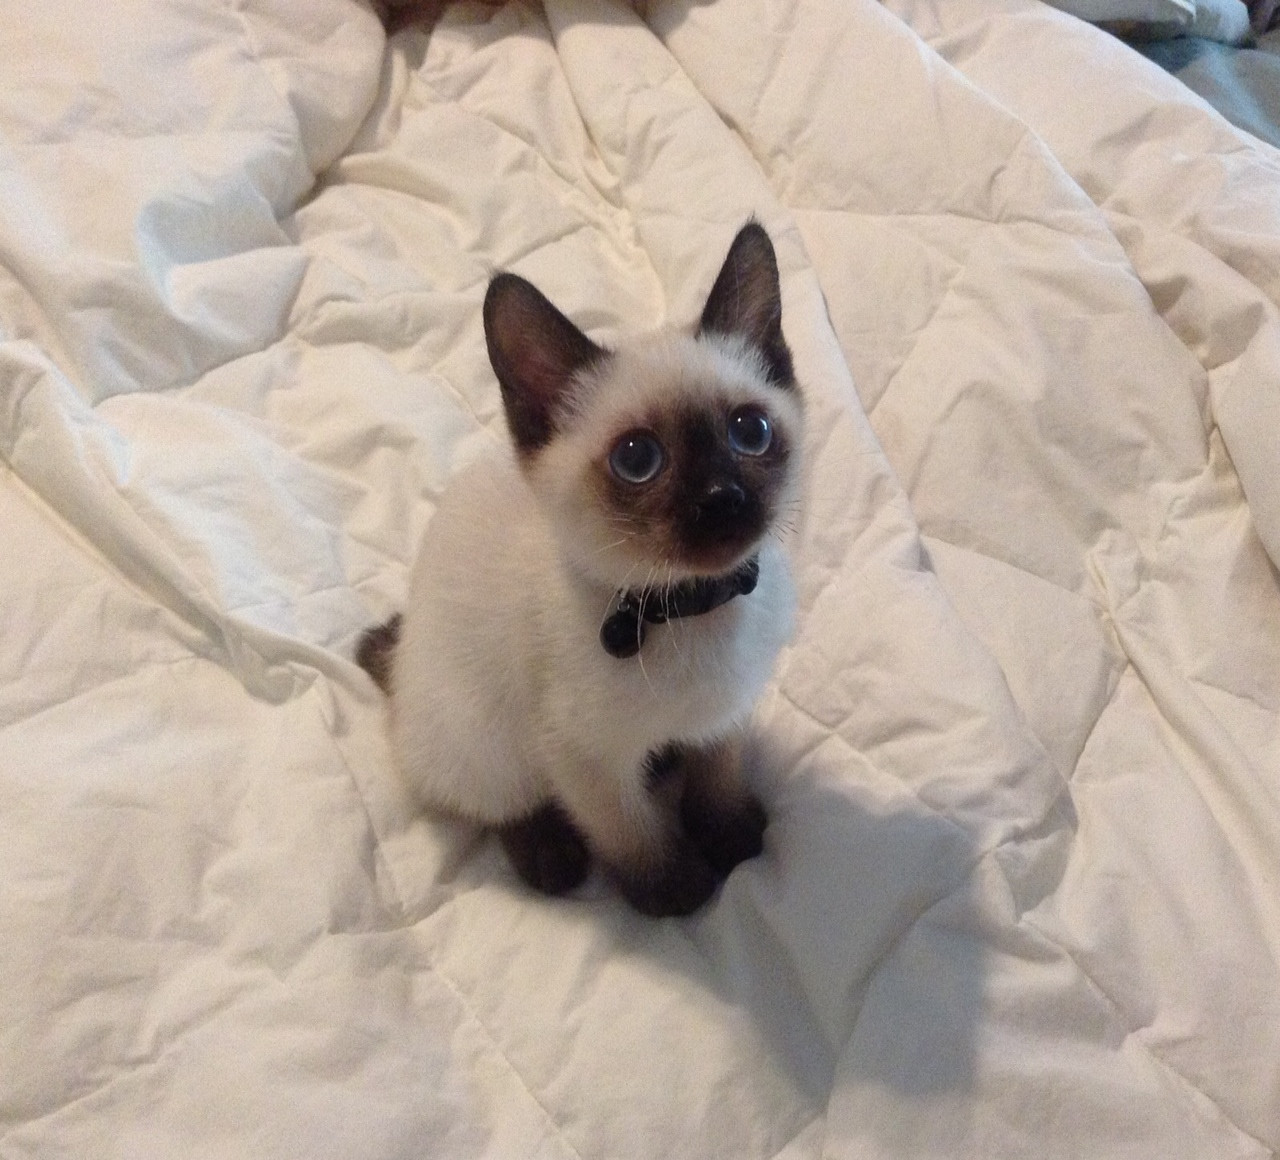
\includegraphics[scale=0.4]{picture.png}
\end{center}

\end{document}
